\documentclass{article}

\usepackage{hyperref}
\usepackage{amsmath}
\usepackage{subcaption}
\usepackage{graphicx}

% Page layout
\hoffset -0in
\voffset -1in
\oddsidemargin 0in
\textheight 9.3in
\textwidth 6.3in

\setlength{\parindent}{0pt}
%\setlength{\intextsep}{10pt}
%\pagestyle{empty}

\graphicspath{{figures/}}

\begin{document}
	\section*{COMPUTATIONAL METHODS IN MECHANICS: Task 2}
	Vesa-Ville Hurskainen, 30 Jan 2018
	
	\section*{Introduction}
	This report concerns assignment two of the course \textit{Computational Methods in Mechanics}, on solving the dynamic response of a mass-spring-damper system using MATLAB. The assignment comprises five tasks.% which are as follows:
	
%	\begin{enumerate}
%		\setlength\itemsep{0pt}
%		\item To use GitHub.
%		\item To create a MATLAB code that solves a mass-spring-damper system.
%		\item To compare the exact solution for free and damped vibrations using different ODE solvers.
%		\item To reduce the error in position by adjusting solver settings.
%		\item To analyze forced and slightly damped vibrations with harmonic force, and investigate what happens when the force frequency passes the damped natural frequency and how the rate of change of the force frequency affects the solution.
%	\end{enumerate}
	
	\section*{Methods}
	Denoting displacement with $x$ and external force with $F$, the equation of motion for the mass-spring-damper system can be written as
	\begin{equation}
		m \ddot{x} + c \dot{x} + k x  = F
	\end{equation}
	where $m$ is mass, $c$ is damping coefficient and $k$ is spring coefficient. In this case, the force is defined as
	\begin{equation}
		F(t) = A \sin(\omega(t) t)
	\end{equation}
	where $A$ is harmonic force amplitude and $\omega$ is frequency. The analytically derived response function of the system, presuming that $F=0$ and system is underdamped (damping ratio $<$ 1), can be written as
	\begin{equation}
		x(t) = e^{-\zeta \omega_n t} \left(\frac{\dot{x}_0 + \zeta \omega_n x_0}{\omega_d} \sin(\omega_d t) + x_0 \cos(\omega_d t)\right)
	\end{equation}
	where damping ratio $\zeta = c / \sqrt{km}$, undamped natural frequency $\omega_n = \sqrt{k/m}$ and damped natural frequency $\omega_d = \omega_n \sqrt{1-\zeta^2}$. The initial values for displacement and velocity are $x_0$ and $\dot{x}_0$, respectively.\\
	
	To compute the required results, two MATLAB scripts were written. The first (\texttt{task2\_solver\_comparison.m}) was written to compare the system responses produced using different ODE solvers to the analytical results, completing tasks two to four. The second script (\texttt{task2\_harmonic\_force.m}) was made to analyze the response of the system with harmonic force, completing task five.
	
	\section*{Results}
	The following system parameters were used: $m$ = 1 kg, $k$ = 100 N/m, $c$ = 0.1 Ns/m. Output time vector was defined as $0:0.01:10$ s. A comparison of undamped and damped system responses with different ODE solvers is presented in Figure~\ref*{fig:response}. Following this, Table~\ref*{tab:error_comparison} presents a comparison between the maximum errors produced by the solvers with two different sets of solver options. Finally, a comparison of the system's forced responses with different frequencies of harmonic force is presented in Figure~\ref*{fig:forced_response}.

	\section*{Analysis}
	The completion of the second and third tasks given in the instructions can be verified from Figure~\ref*{fig:response}. The numerical and analytical solutions coincide with a fair degree of accuracy in all cases, but consistently the best results were gained using the solver ode45 and the worst using ode23. The completion of task four can be verified from Table~\ref*{tab:error_comparison}, which shows a significant decrease in error with tighter tolerances.\\
	
	The fifth task required comparing the forced response of the system with different parameters, which can be done using Figure~\ref*{fig:forced_response}. The figure shows that following the force frequency passing $\omega_d$, the vibration of the system begins to subside. Before this, the amplitude rises. It is also shows that raising the rate of frequency change both makes the transition happen earlier (naturally) and causes the maximum amplitude to be lower. \\
	
	The first task was completed by uploading the employed scripts and the source files of this report into a \href{https://github.com/VesaVilleHurskainen/cmim2018}{GitHub repository} using the MATLAB-integrated functions. Therefore, all five tasks are judged to be complete.
	
	\clearpage
		\begin{figure}[h]
		\centering
		\begin{subfigure}[t]{0.41\textwidth}
			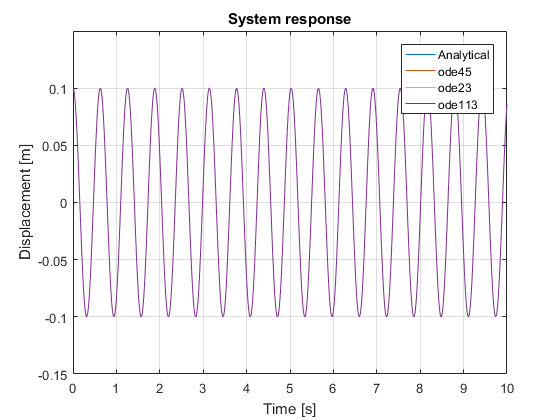
\includegraphics[width=\textwidth]{response_comparison_undamped.png}
			\caption{Response, $\zeta = 0$ .}
		\end{subfigure}
		~
		\begin{subfigure}[t]{0.41\textwidth}
			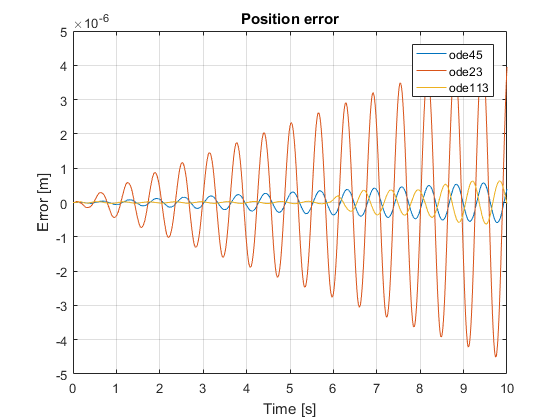
\includegraphics[width=\textwidth]{error_comparison_undamped.png}
			\caption{Position error, $\zeta = 0$ .}
		\end{subfigure}
		
		\begin{subfigure}[t]{0.41\textwidth}
			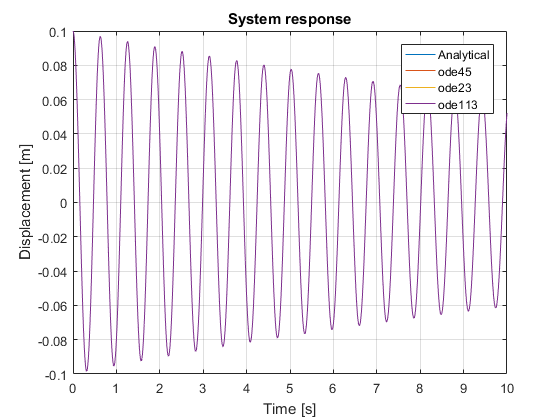
\includegraphics[width=\textwidth]{response_comparison_damped.png}
			\caption{Response, $\zeta = 0.1$ .}
		\end{subfigure}
		~
		\begin{subfigure}[t]{0.41\textwidth}
			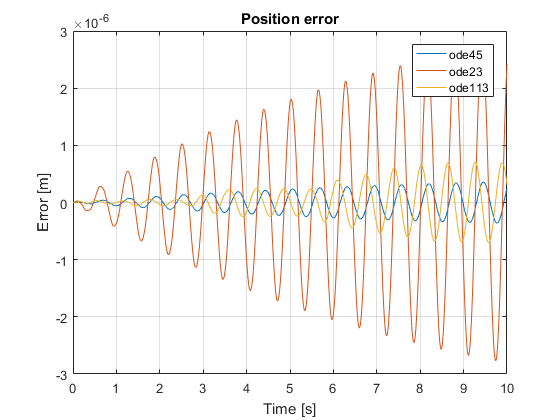
\includegraphics[width=\textwidth]{error_comparison_damped.png}
			\caption{Position error, $\zeta = 0.1$ .}
		\end{subfigure}
		\caption{System response comparison, undamped and damped cases. Default solver options.}
		\label{fig:response}
	\end{figure}
	
	\begin{table}[h]
		\centering
		\def\arraystretch{1.1}
		\caption{Comparison of maximum errors [$10^{-6}$ m].}
		\begin{subtable}[t]{0.4\textwidth}
			\centering
			\caption{Default options.}
			\begin{tabular}{|l|l|l|}
				\hline
				Solver & $\zeta = 0$ & $\zeta = 0.1$\\
				\hline
				ode45  & 1016 & 621.4 \\
				ode23  & 5042 & 3100 \\
				ode113 & 1482 & 953.4 \\
				\hline
			\end{tabular}
		\end{subtable}
		~
		\begin{subtable}[t]{0.4\textwidth}
			\centering
			\caption{AbsTol = 1e-9, RelTol = 1e-3 .}
			\begin{tabular}{|l|l|l|}
				\hline
				Solver & $\zeta = 0$ & $\zeta = 0.1$\\
				\hline
				ode45  & 0.5887 & 0.3609 \\
				ode23  & 4.506 & 2.770 \\
				ode113 & 0.6283 & 0.7028 \\
				\hline
			\end{tabular}
		\end{subtable}
		\label{tab:error_comparison}
	\end{table}
	
	\begin{figure}[h!]
		\centering
		\begin{subfigure}[t]{0.41\textwidth}
			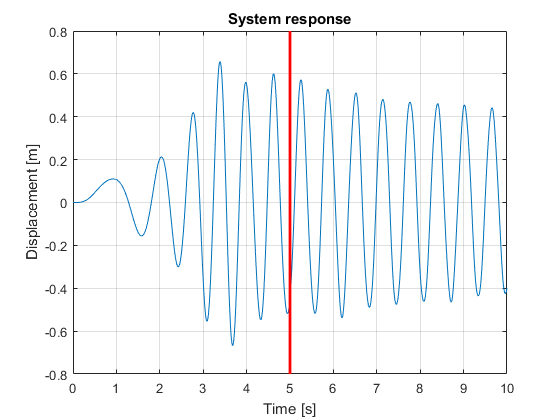
\includegraphics[width=\textwidth]{forced_response_slow.png}
			\caption{Response, $\omega = 2 t$ .}
		\end{subfigure}
		~
		\begin{subfigure}[t]{0.41\textwidth}
			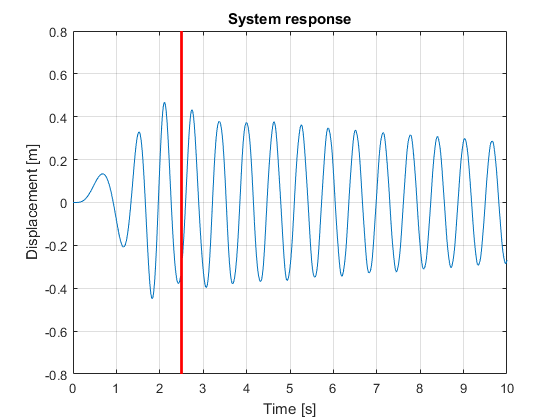
\includegraphics[width=\textwidth]{forced_response_fast.png}
			\caption{Response, $\omega = 4 t$ .}
		\end{subfigure}
		\caption{Forced response, $A$ = 10 N, $\zeta$ = 0.1 . Solver ode45, default options. Vertical line = $\omega_d$.}
		\label{fig:forced_response}
	\end{figure}
\end{document}